\section{Pengantar Kriptografi Kunci-Publik}
\label{sec:pengantar-kunci-publik}

Kriptografi kunci-publik, atau kriptografi asimetris, adalah sistem yang menggunakan
sepasang kunci yang berbeda: \textbf{kunci publik} (\textit{public key}) dan \textbf{kunci
privat} (\textit{private key}). Kunci publik dapat disebarkan secara terbuka, sementara
kunci privat harus dijaga kerahasiaannya oleh pemiliknya. Yang membuat gagasan ini
revolusioner bukan sekadar jumlah kuncinya yang lebih sedikit, melainkan bahwa dua orang
yang belum pernah bertemu dan tidak memiliki saluran rahasia sama sekali tetap dapat
bertukar pesan rahasia.

\subsection{Masalah Distribusi Kunci pada Kriptografi Simetris}

Seluruh bab-bab sebelumnya membahas algoritma yang memakai \emph{satu} kunci untuk
enkripsi dan dekripsi. Kekuatan AES, misalnya, tidak ada gunanya bila kunci yang
dipakainya harus dikirim lebih dahulu kepada penerima. Pengirim dan penerima harus
menyepakati kunci itu melalui saluran yang aman --- tetapi saluran yang aman itulah yang
justru ingin dibangun. Keadaan ini disebut \textbf{masalah distribusi kunci}
(\textit{key distribution problem}), dan sampai pertengahan dekade 1970-an ia dianggap
sebagai bagian tak terhindarkan dari setiap sistem kriptografi.

Masalah itu menjadi semakin berat seiring bertambahnya jumlah pengguna. Bila $n$ orang
saling berkomunikasi secara rahasia dan setiap pasangan memerlukan kunci tersendiri, maka
jumlah kunci yang harus dibangkitkan, disalurkan, dan disimpan adalah

\[
\binom{n}{2} = \frac{n(n-1)}{2}.
\]

Untuk sepuluh pengguna dibutuhkan 45 kunci, untuk seratus pengguna 4.950 kunci, dan untuk
seribu pengguna hampir setengah juta kunci. Setiap kunci tambahan adalah satu titik yang
dapat bocor, sehingga pertumbuhan kuadratik ini bukan sekadar persoalan penyimpanan,
melainkan persoalan keamanan yang mendasar.

\subsection{Fungsi Satu Arah dan Pintu Jebakan}

Landasan matematis kriptografi kunci-publik adalah keberadaan fungsi yang mudah dihitung
satu arah tetapi praktis mustahil dibalik. Konsep dasarnya dirumuskan sebagai berikut.

\begin{definition}[Fungsi satu arah]
Suatu fungsi $f$ disebut \textbf{fungsi satu arah} (\textit{one-way function}) jika untuk
setiap $x$ di daerah asalnya, nilai $f(x)$ dapat dihitung dalam waktu polinomial, tetapi
untuk hampir setiap nilai $y$ di daerah hasilnya, mencari $x$ sedemikian sehingga
$f(x) = y$ memerlukan waktu yang tidak praktis.
\end{definition}

Fungsi satu arah saja belum cukup untuk berkirim pesan. Penerima yang sah harus tetap
dapat membalik prosesnya, sedangkan penyerang tidak. Karena itu diperlukan fungsi yang
mempunyai jalan rahasia di dalamnya.

\begin{definition}[Fungsi satu arah dengan pintu jebakan]
Suatu fungsi satu arah $f$ disebut \textbf{fungsi satu arah dengan pintu jebakan}
(\textit{trapdoor one-way function}) jika terdapat informasi rahasia $t$ sedemikian
sehingga $f$ dapat dibalik dengan mudah apabila $t$ diketahui, tetapi tetap tidak praktis
dibalik tanpa $t$.
\end{definition}

Pada RSA, fungsinya adalah pemangkatan modulo $n$, informasi rahasianya adalah faktorisasi
$n$ (yaitu $p$ dan $q$ itu sendiri), dan tanpa informasi itu membalik fungsi tersebut
setara dengan memfaktorkan modulus yang telah dipilih sangat besar.

Perbedaan pokok kriptografi simetris dan asimetris dirangkum pada
Tabel~\ref{tab:simetris-vs-asimetris}.

\begin{table}[htbp]
    \centering
    \caption{Perbandingan kriptografi simetris dan asimetris}
    \label{tab:simetris-vs-asimetris}
    \begin{tabularx}{\linewidth}{|l|>{\raggedright\arraybackslash}X|>{\raggedright\arraybackslash}X|}
    \hline
    \textbf{Aspek} & \textbf{Simetris} & \textbf{Asimetris} \\
    \hline
    Jumlah kunci & Satu kunci untuk enkripsi dan dekripsi & Sepasang kunci: publik dan privat \\
    \hline
    Distribusi kunci & Kunci harus disalurkan melalui saluran aman & Kunci publik boleh disebarkan terbuka \\
    \hline
    Kecepatan & Cepat, cocok untuk data berukuran besar & Lambat, umumnya untuk kunci dan tanda tangan \\
    \hline
    Contoh algoritma & DES, AES, RC4 & RSA, ElGamal, ECC \\
    \hline
    Kebutuhan kunci bagi $n$ pengguna & Sekitar $n(n-1)/2$ kunci rahasia & $2n$ kunci (publik dan privat) \\
    \hline
    Bukti keaslian asal & Tidak dapat diperiksa tanpa kunci bersama & Dapat, melalui tanda tangan digital \\
    \hline
    \end{tabularx}
\end{table}

\subsection{Kerahasiaan Komponen Algoritma RSA}

Algoritma RSA (Rivest-Shamir-Adleman), yang diperkenalkan pada tahun 1978
\citep{rsa1978}, merupakan salah satu implementasi kunci-publik yang paling fundamental
dan banyak digunakan di dunia. Bab ini memakai delapan lambang yang perannya harus
dibedakan dengan cermat sejak awal, sebab sebagian besar kesalahan penggunaan RSA berasal
dari mencampuradukkan yang rahasia dengan yang boleh diketahui publik.
Tabel~\ref{tab:properti-rsa} merangkum kedudukannya.

\begin{table}[htbp]
    \centering
    \begin{tabularx}{\linewidth}{@{}c >{\raggedright\arraybackslash}X c@{}}
    \toprule
    \textbf{Lambang} & \textbf{Arti} & \textbf{Kerahasiaan} \\
    \midrule
    $p, q$      & Dua bilangan prima pembentuk modulus & Rahasia \\
    $n = p \cdot q$ & Modulus, panjangnya menentukan ukuran kunci & Umum \\
    $\varphi(n)$ & Fungsi Totient Euler, $\varphi(n)=(p-1)(q-1)$ & Rahasia \\
    $e$         & Eksponen enkripsi, disebut kunci publik & Umum \\
    $d$         & Eksponen dekripsi, disebut kunci privat & Rahasia \\
    $m$         & Plainteks, yaitu pesan yang dikirim & Rahasia \\
    $c$         & Cipherteks, yaitu hasil enkripsi & Umum \\
    \bottomrule
    \end{tabularx}
    \caption{Komponen algoritma RSA dan kedudukannya. Pasangan $(e, n)$ adalah kunci
    publik, sedangkan pasangan $(d, n)$ adalah kunci privat}
    \label{tab:properti-rsa}
    \sumber{Munir, \textit{IF4020 Kriptografi}, ITB.}
\end{table}

Dua hal pada tabel itu sering disalahpahami. Pertama, modulus $n$ bersifat umum pada
kedua kunci, sehingga membocorkan $n$ bukan pelanggaran keamanan --- yang harus dijaga
adalah faktor-faktornya. Kedua, $\varphi(n)$ tidak pernah dikirimkan ke mana pun; nilainya
hanya dipakai sekali saat pembangkitan kunci, lalu dibuang. Penyerang yang berhasil
memperoleh $\varphi(n)$ dapat menghitung $d$ dalam waktu sekejap, sehingga kerahasiaan
$\varphi(n)$ sama pentingnya dengan kerahasiaan $d$ itu sendiri.

\begin{figure}[htbp]
    \centering
    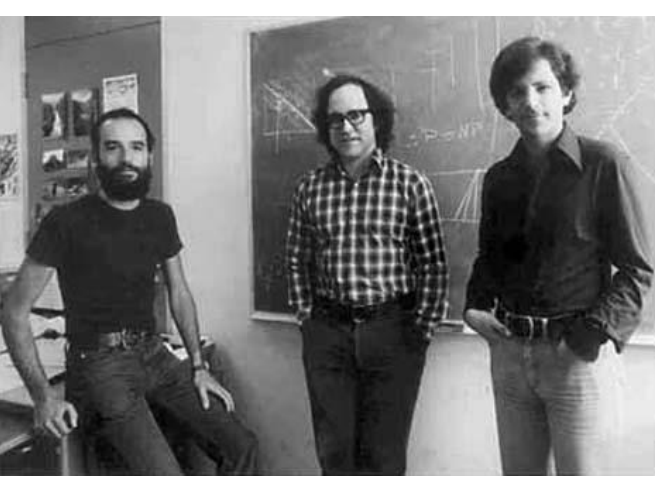
\includegraphics[width=0.7\linewidth, height=0.45\textheight, keepaspectratio]{figures/penemu-rsa.png}
    \caption{Ron Rivest, Adi Shamir, dan Len Adleman, para perumus algoritma RSA}
    \label{fig:penemu-rsa}
    \sumber{Munir, \textit{IF4020 Kriptografi}, ITB.}
\end{figure}

\subsection{Sejarah Singkat Algoritma RSA}

Gagasan kriptografi kunci-publik pertama kali dipublikasikan oleh Whitfield Diffie dan
Martin Hellman pada 1976 \citep{diffie1976}, tetapi mereka belum memberikan skema
enkripsi yang lengkap: protokol mereka hanya memungkinkan dua pihak menyepakati kunci
rahasia, bukan mengirim pesan. Skema enkripsi pertama yang utuh baru muncul setahun
kemudian dari tiga peneliti di \textit{Massachusetts Institute of Technology}, yaitu
Ronald Rivest, Adi Shamir, dan Leonard Adleman, dan diterbitkan pada Februari 1978 di
jurnal \textit{Communications of the ACM} \citep{rsa1978}.

Nama RSA sendiri disusun dari huruf awal ketiga nama belakang mereka. Urutan namanya
ditentukan oleh sebuah kebetulan administratif: Rivest menyusun makalahnya secara
alfabetis, dan sejak itu urutan tersebut melekat pada nama algoritmanya, meskipun
sumbangan pemikiran Shamir dan Adleman sama besarnya.

Kepercayaan pada RSA tumbuh melalui uji publik yang panjang. Pada 1977, majalah
\textit{Scientific American} memuat angka 129 digit sebagai tantangan berhadiah \$100;
tantangan itu baru terpecahkan pada 1994 setelah sekitar 600 sukarelawan dari 24 negara
bekerja bersama melalui jaringan Internet selama delapan bulan \citep{atkins1995rsa129}.
Kemenangan atas modulus 129 digit itu menutup satu era: sejak saat itu panjang kunci RSA
yang dianggap aman terus bertambah, dan sejarah itu diuraikan lebih rinci pada
Subbagian~\ref{subsec:kesulitan-pemfaktoran}.

Satu catatan administratif yang penting bagi pengguna: algoritma RSA pernah dilindungi
paten di Amerika Serikat dari 1983 sampai 2000. Setelah paten itu berakhir, RSA menjadi
milik umum dan tersedia bebas di perpustakaan kriptografi mana pun.

\subsection{Kedudukan RSA dalam Kriptografi Modern}

RSA bukan pengganti algoritma kunci-simetri, melainkan pelengkapnya. Perbedaan kecepatan
antara keduanya sangat besar --- RSA pada perangkat lunak umumnya ratusan sampai ribuan
kali lebih lambat daripada AES untuk jumlah data yang sama --- sehingga pembagian tugas
di antara keduanya menjadi baku:

\begin{itemize}
    \item RSA dipakai untuk hal-hal yang datanya pendek tetapi menuntut keamanan
          jangka panjang: menyalurkan kunci sesi bersama protokol
          Diffie--Hellman (Bab~\ref{chap:diffie-hellman}) maupun ElGamal
          (Bab~\ref{chap:elgamal}), serta membuat tanda tangan digital
          (Bab~\ref{chap:tanda-tangan-pki}).
    \item AES dan kerabatnya dipakai untuk mengenkripsi data berukuran besar, memakai
          kunci sesi yang telah disalurkan oleh RSA.
\end{itemize}

RSA juga menjadi induk bagi seluruh keluarga algoritma kunci-publik lainnya. ElGamal
(Bab~\ref{chap:elgamal}) memakai gagasan yang sama dengan operasi pemangkatan pada grup
siklik, sedangkan kriptografi kurva eliptik (Bab~\ref{chap:ecc}) memindahkan operasi itu
ke himpunan titik pada kurva sehingga ukuran kuncinya dapat dipersingkat. Dengan
memahami RSA terlebih dahulu, pola penalaran yang dipakai oleh seluruh keluarga algoritma
tersebut --- pilih masalah matematis yang sukar dibalik, rahasiakan pintu jebakannya,
umumkan petunjuknya --- akan terlihat jelas.
